\subsection{Conversão para Monocromático}

A transformação para escala de cinza é feita através da média dos três canais de cores, truncada para inteiro. A matriz resultante é então repetida novamente para os três canais, para que a operação possa ser repetida sem erros de execução do programa.

\begin{figure}[H]
    \centering
    \begin{subfigure}{0.45\textwidth}
        \centering
        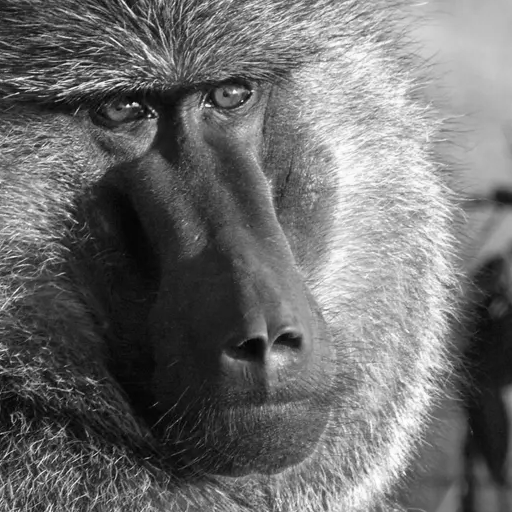
\includegraphics[width=6cm]{resultados/colormono.png}
        \caption{\texttt{imagens/color.png}}
    \end{subfigure}%
    \begin{subfigure}{0.45\textwidth}
        \centering
        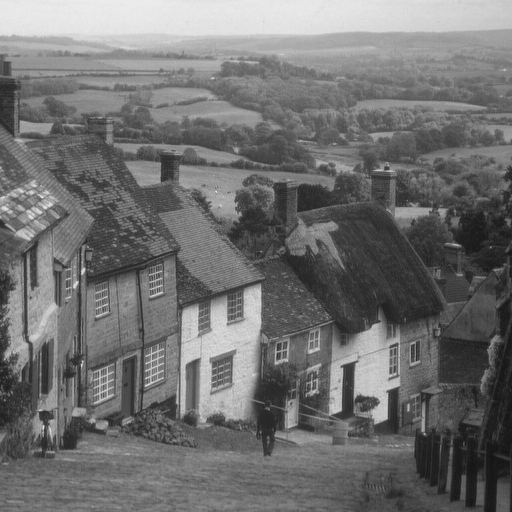
\includegraphics[width=6cm]{resultados/citymono.png}
        \caption{\texttt{imagens/city.png}}
        \label{fig:res:1}
    \end{subfigure}

    \caption{Imagem em escala de cinza.}
\end{figure}

\begin{listing}[htb]
    \caption{Comando \texttt{monocromatico}}

    \begin{minted}{python}
        def grayscale(imagem):
            gray = np.mean(imagem, axis=2).astype(np.uint8)
            return np.stack([gray, gray, gray], axis=2)
    \end{minted}
\end{listing}

Em vez de \pyline{np.mean(imagem, ...)}, a conversão poderia ser implementado também com \pyline{cv2.cvtColor(imagem, cv2.COLOR_BGR2GRAY)} \autocite{ref:cvtcolor}.
